\subsection{Biological testing\label{sec:bio1}}

\subsubsection{Autoinducer-antibiotic conjugates}

The eight triazoles made in \ref{sec:Tris} (see \ref{fgr:finals_1}) were tested for antibacterial and anti-biofilm activity in \textit{P. aeruginosa} PAO1\cite{Stover2000} and YM64\cite{Morita2001}.

\begin{figure}[H]
	\begin{center}
		\schemeref[HL2T4Cip]{cmpd:HL2T4Cip}
		\schemeref[HL4T4Cip]{cmpd:HL4T4Cip}
		\schemeref[HL6T4Cip]{cmpd:HL6T4Cip}
		\schemeref[6HHQT4Cip]{cmpd:6HHQT4Cip}
		\schemeref[HL4T4Tri]{cmpd:HL4T4Tri}
		\schemeref[HL6T4Tri]{cmpd:HL6T4Tri}
		\schemeref[6HHQT4Tri]{cmpd:6HHQT4Tri}
		\schemeref[PQST4Tri]{cmpd:PQST4Tri}	
		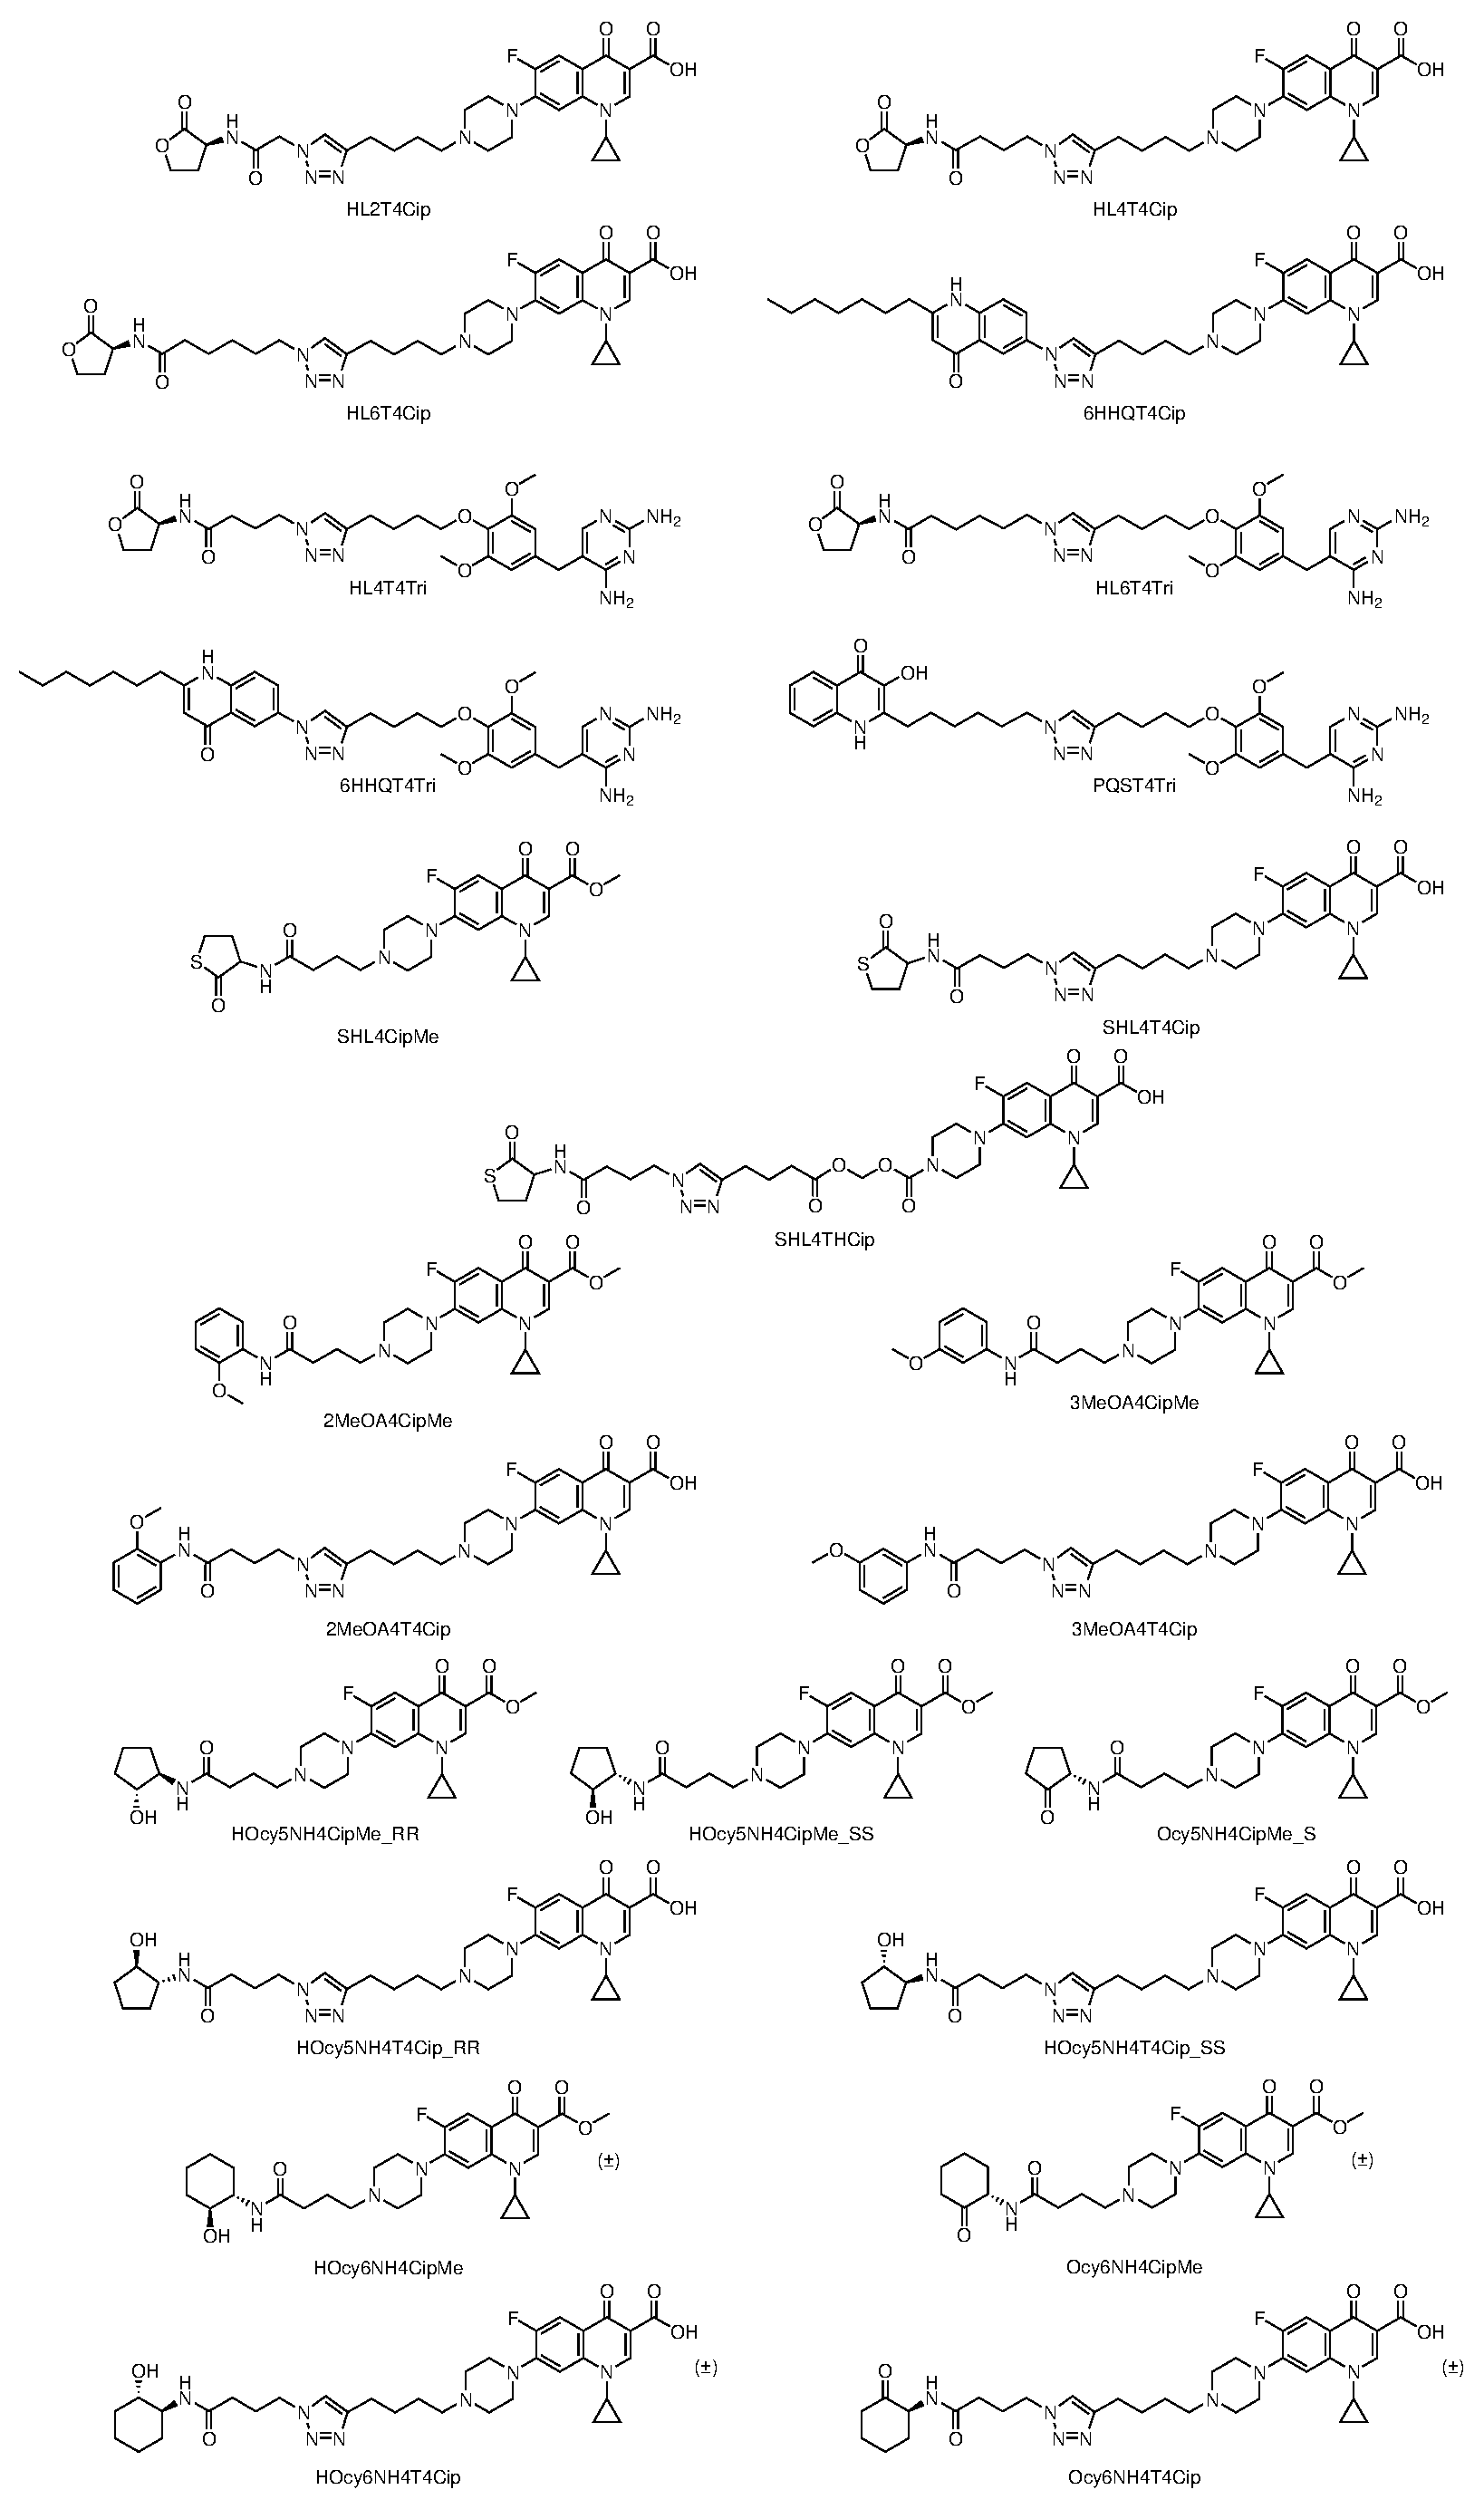
\includegraphics[width=\textwidth]{finals_1}
		\caption{
 		\label{fgr:finals_1}}
	\end{center}
\end{figure}


In YM64 at 5 h the HSL-ciprofloxacin conjugates \compound{cmpd:HL2T4Cip}, \compound{cmpd:HL4T4Cip} and \compound{cmpd:HL6T4Cip} showed slight activity at the highest concentration, but not as much as ciprofloxacin \compound{cmpd:Cip}.
This activity was not visible by 24 h (see \ref{fgr:YM64_24h}) and the compounds had no effect on biofilm formation (see \ref{fgr:YM64_biofilms}).


\begin{figure}[H]
	\begin{center}
		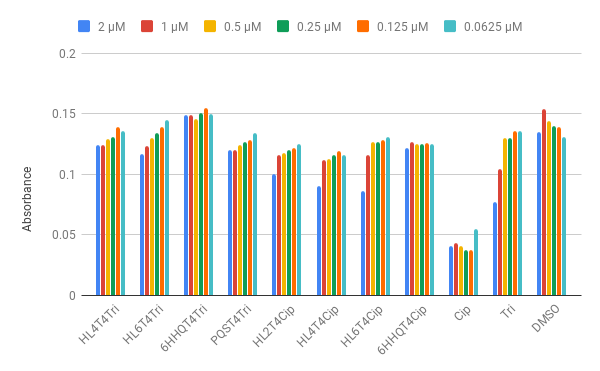
\includegraphics[width=\textwidth]{YM64_5h}
		\caption{YM64 5 h.\label{fgr:YM64_5h}}
	\end{center}
\end{figure}

\begin{figure}[H]
	\begin{center}
		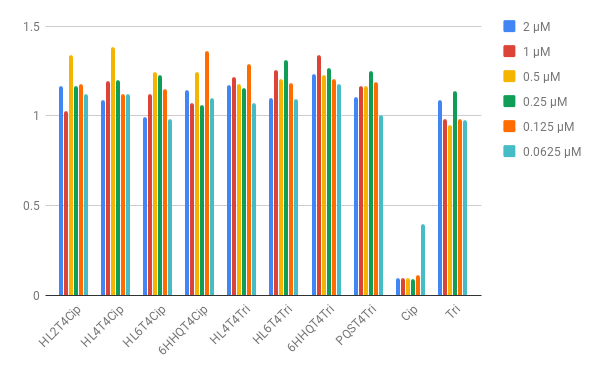
\includegraphics[width=\textwidth]{YM64_24h}
		\caption{YM64 24 h.\label{fgr:YM64_24h}}
	\end{center}
\end{figure}

\begin{figure}[H]
	\begin{center}
		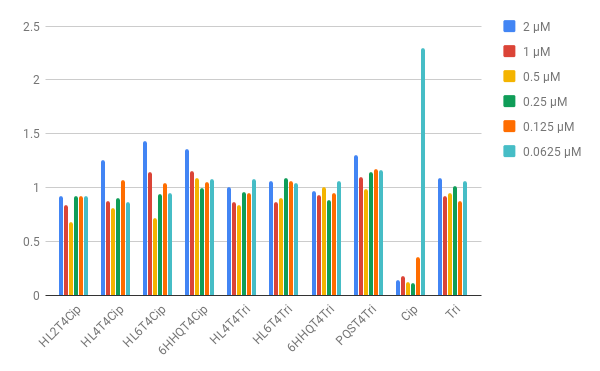
\includegraphics[width=\textwidth]{YM64_biofilms}
		\caption{YM64 biofilms 24 h.\label{fgr:YM64_biofilms}}
	\end{center}
\end{figure}

In PAO1 \compound{cmpd:HL6T4Cip} showed similar activity to ciprofloxacin \compound{cmpd:Cip} at the highest concentration (see \ref{fgr:PAO1_5h}), but not at lower concentrations. All other compounds did not show activity, and again there was no activity at 24 h or against biofilms.

\begin{figure}[H]
	\begin{center}
		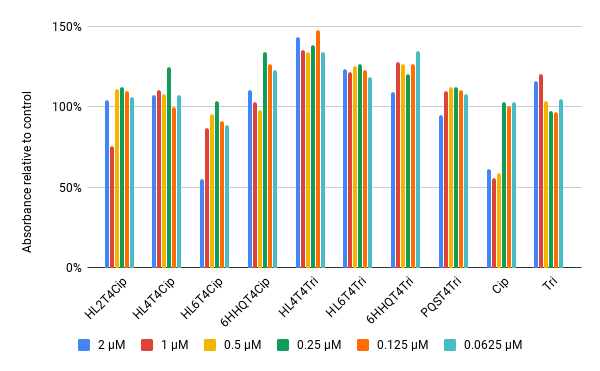
\includegraphics[width=\textwidth]{PAO1_5h}
		\caption{PAO1 5 h.\label{fgr:PAO1_5h}}
	\end{center}
\end{figure}

\begin{figure}[H]
	\begin{center}
		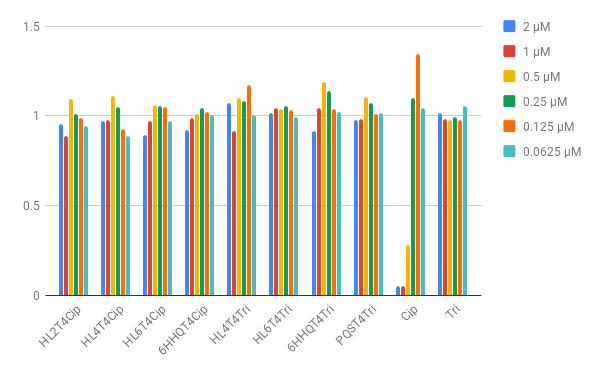
\includegraphics[width=\textwidth]{PAO1_24h}
		\caption{PAO1 24 h.\label{fgr:PAO1_24h}}
	\end{center}
\end{figure}

\begin{figure}[H]
	\begin{center}
		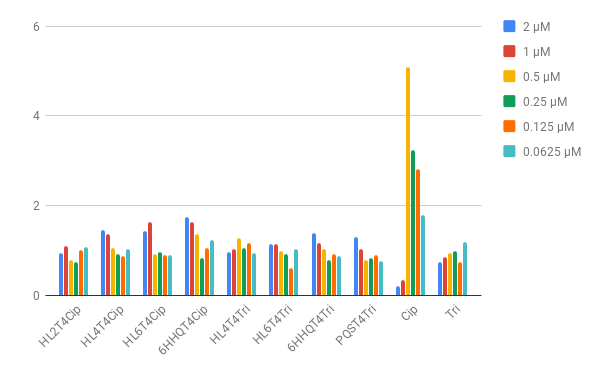
\includegraphics[width=\textwidth]{PAO1_biofilms}
		\caption{PAO1 biofilms 24 h.\label{fgr:PAO1_biofilms}}
	\end{center}
\end{figure}

\subsubsection{Cleavable HSL-ciprofloxacin conjugates}

The eight cleavable HSL-ciprofloxacin conjugates, two controls and two alkynes described in \ref{sec:cleavable} (see \ref{fgr:finals_cleavable}) were tested for antibacterial and anti-biofilm activity in \textit{P. aeruginosa} YM64. 

\begin{figure}[H]
	\begin{center}
		\schemeref[HL2THCip]{cmpd:HL2THCip}
		\schemeref[HL4THCip]{cmpd:HL4THCip}
		\schemeref[HL6THCip]{cmpd:HL6THCip}
		\schemeref[HL2TMeCip]{cmpd:HL2TMeCip}
		\schemeref[HL4TMeCip]{cmpd:HL4TMeCip}
		\schemeref[HL6TMeCip]{cmpd:HL6TMeCip}
		\schemeref[BnTHCip]{cmpd:BnTHCip}
		\schemeref[BnTMeCip]{cmpd:BnTMeCip}		
		\schemeref[Y4HCip]{cmpd:Y4HCip}
		\schemeref[Y4MeCip]{cmpd:Y4MeCip}
		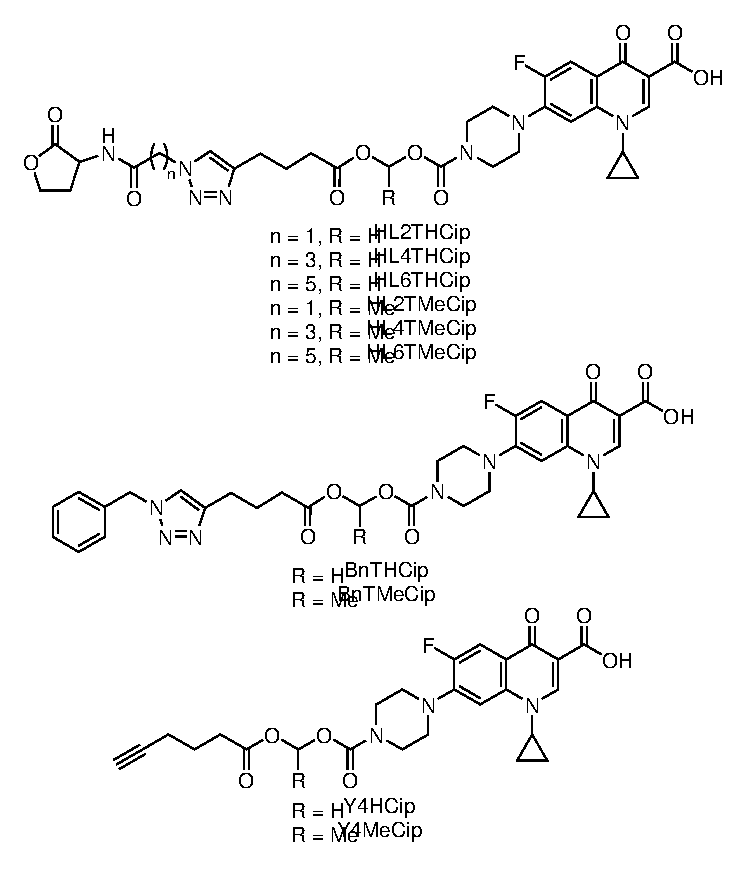
\includegraphics[scale=1]{finals_cleavable}
		\caption{
 		\label{fgr:finals_cleavable}}
	\end{center}
\end{figure}

Here there was more success, although the activity was still not as high as for ciprofloxacin \compound{cmpd:Cip}.
The HSL-ciprofloxacin conjugates with \textit{N}-(acetoxymethoxycarbonyl) linkers (R = H) showed activity at high concentrations. A longer linker seems to give higher activity; \compound{cmpd:HL4THCip} and \compound{cmpd:HL6THCip} showed activity comparable with ciprofloxacin \compound{cmpd:Cip} at high concentrations.
Unfortunately the control \compound{cmpd:BnTHCip} and alkyne \compound{cmpd:Y4HCip} with \textit{N}-(acetoxymethoxycarbonyl) linkers (R = H) showed higher activity than the conjugates, indicating that the HSL head wasn't contributing to the activity of the conjugates.

The conjugates with an \textit{N}-(acetoxyethoxycarbonyl) linker (R = Me) did not show any activity. This suggests that they either didn't enter cells or weren't suitable substrates for esterases.
The \textit{N}-(acetoxyethoxycarbonyl) linked alkyne (R = Me) did show some activity, indicating that maybe it could penetrate cells more easily than the conjugates due to its lower molecular weight and/or lower polarity.

\begin{figure}[H]
	\begin{center}
		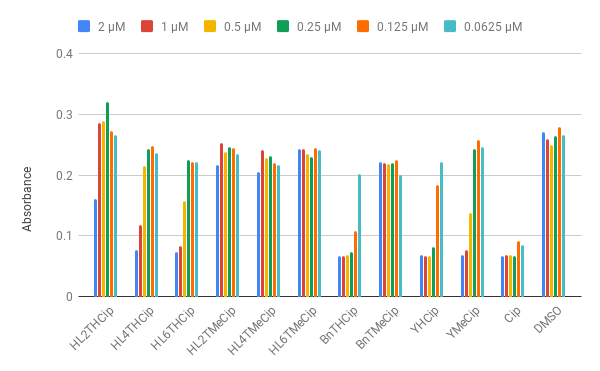
\includegraphics[width=\textwidth]{YM64_5h_cleavable}
		\caption{YM64 5 h cleavable conjugates.\label{fgr:YM64_5h_cleavable}}
	\end{center}
\end{figure}
